\chapter{Požadavky}
voděodolnost


\chapter{Základní návrh}
%tady musí být text
%bude tady také blokové schéma

\section{Mikrokontrolér}

\section{LED}
Jendím z nejdůležitějších požadavků na Semafor je, aby mohl svítit. Čím více možností, jak svítit, tím bude využití 
při hrách a táborových programech větší. K tomu jsou použity LED. Obyčejné LED mají pouze jednu barvu, kterou 
mohou svítit. Existují také RBG LED, ale ty mají 4 vývody a každá LED tak zabírá 3 GPIO piny mikrokontroléru - jeden pin
pro jednu barvu. K tomu by byl zapotřebí mikrokonrolér s velkým množství GPIO pinů a jeho programování by se tím značně 
komplikovalo. Ani to není žádoucí, a proto byly použity programovatelné LED typu WS2812C. %citace

%způsob programování (jak funguje použitá knihovna?)

Tyto programovatelné LED WS2812C lze spojovat za sebe, takže datový výstup jedné LED je připojen k datovému vstupu další LED %citace
Takto lze spojit nekonečné množství těchto programovatelných LED. 

%obrázek spojení LED za sebe

%napsat o jejich spotřebě
%spočítat, jakou budou mít spotřebu celkem (všech 12) při bílé

%do sekce o DPS se zmínit o jejich umístění - kruh, hodiny, proto 12 ks. (lze také rozdělit na 3 segmenty)

\section{Tlačítka}
Tlačítka mohou být realizována dvěma základními způsoby, mohou být elektromechanická, nebo kapacitní dotyková. 

Dotyková plocha mechanického tlačítka je nevodivá, často plastová. 

Mechanické tlačítko typu NO: %upravit

Po zmáčknutí mechanického tlačítka jsou 2 kovové části tlačítka spojeny, tím dochází ke spojení elektrického obvodu 
a odpor smyčky je v ideálním případě nulový. Tlačítko je tedy sepnuto. Když je tlačítko rozpojeno, tak je 
elektrický obvod přerušen a odpor smyčky je v ideálním případě nekonečný.

Mechanické tlačítko typu NC: %upravit

U tlačítka NC je to přesně naopak. %upravit

%sem přidat fotku vnitřku mechanického tlačítka

Kapacitní tlačítka jsou tvořena měděnou vrstvou (nejčastěji spirálou) a nejsou nijak mechanicky namáhána.


\subsection{Princip kapacitních dotykových tlačítek}
Základní princip je založen na měření změny kapacity. Měď, ze které je tlačítko vytvořeno má
nějakou vlastní kapacitu (kapacita samotné nosné desky) a po přiložení prstu je kapacita zvýšena o paralelně 
připojenou kapacitu přechodu tlačítka a prstu díky obsahu železa v krvi a vodivosti kůže \cite{PrincipKapTl}. 
Prst se tedy chová jako druhá uzemněná elektroda \cite{PrincipKapTl}. 

Kapacita snímače se tedy volí co nejmenší, aby přiložený prst vyvolal co nejvetší změnu kapacity. Ve snímači se vyskytuje
RC článek, kterého se mění doba nabíjení kondenzátoru a tím je možné detekovat stisk tlačítka \cite{PrincipKapTl}. 

\subsection{Návrh kapacitního dotykového tlačítka}
Tvar tlačítka nemá vliv na schopnost detekce dotyku \cite{PrincipKapTl}. Naopak velký vliv má plocha tlačítka, tloušťka
izolační vrstvy, a také vzdálenost jednotlivých tlačítek od sebe \cite{PrincipKapTl}. 

Čím větší je plocha tlačítka, tím je větší změna kapacity při dotyku a díky tomu je vytvořena lepší schopnost detekce 
dotyku \cite{PrincipKapTl}. S rostoucí tloušťkou izolační vrstvy se naopak schopnost detekce dotyku snižuje \cite{PrincipKapTl}.

Pokud jsou tlačítka příliš blízko u sebe, tak může docházet k jejich vzájemnému ovlivňování. Kvůli tomu pak může docházet k
detekci dotyku špatného tlačítka, nebo k falešné detekci dotyku. Z doporučení plyne, že pro dotyk prstu je vhodná velikost snímací 
plochu pro prst 13~$\times$~13 mm a jejich vzdálenost alespoň 5 mm od sebe \cite{PrincipKapTl}. Proti vzájemnému ovlivňování tlačítek
se používají uzemňovací meziplošky \cite{PrincipKapTl}.

%sem dát obrázek, kde je ukázán návrh GND meziplošek

U kapacitních dotykových tlačítek je zapotřebí dbát na správné připojení k MCU. U vícevrstvých DPS nesmí pod tlačítky, ani pod přívody
k MCU, vést jiné dráhy, ani se zde nesmí vyskytovat jiné součástky \cite{PrincipKapTl}. Součástky nesmí být ani z vrchní, ani ze spodní 
strany DPS \cite{PrincipKapTl}.

Voda a další nečistoty mění vlastní kapacitu tlačítka a může tak docházet k falešným stiskům tlačítka. Tento problém lze řešit softwarově. 
Lze využít faktu, že nečistoty působí dlouhodobě, ale stisk je krátkodobý \cite{PrincipKapTl}. Hodnotu vlastní kapacity tlačítka je tedy
možné softwarově upravovat v závislosti na aktuálních dlouhodobějších stavech a detekovat tak přesněji krátkodobý stisk tlačítka. 

%že jsem zvolila kapacitní tlačítka a proč


%dát do zkratek MCU, DPS, GPIO



\begin{figure}[!h]
    \begin{center}
      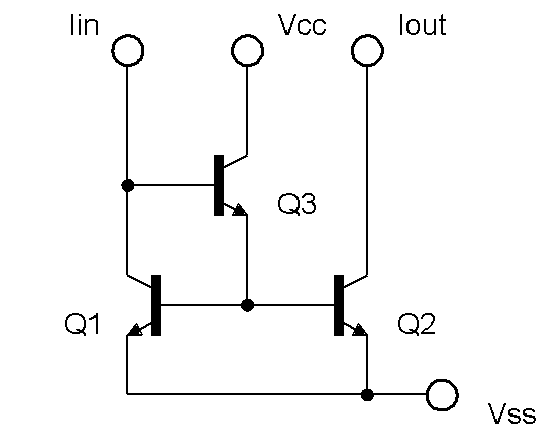
\includegraphics[scale=0.5]{obrazky/ZlepseneWilsonovoZrcadloNPN}
    \end{center}
    \caption[Alenčino zrcadlo]{Zlepšené Wilsonovo proudové zrcadlo.}
  \end{figure}

Pro odlišení tlačítek je místo označeno barevným potiskem. 

\section{Baterie}
Ve výběru baterií hraje velkou roli kapacita, napětí, velikost a cena. Požadavkem je také možnost nabíjení, protože není žádoucí, aby si uživatel
baterie měnil. Při použití na táboře by také musely být stále nové baterie v balení a musely by se neustále doplňovat a udržovat.

Vybraný mikrokonrolér má napájecí napětí v rozsahu 3 až 3,6 V \cite{ESP_C3_dtsh}. 

Z nabíjecích baterií je možno vybírat z nabíjecích tužkových baterií (Ni-MH), Li-Ion, Li-Pol a LiFePO4 baterií.
%Ni-MH
Baterie Ni-MH mají jmenovité napětí 1,25 V, proto by bylo zapotřebí alespoň 3 článků spojených sériově, u kterých by navíc musel být stabilizátor
na 3,3 V pro napájení mikrokontroléru. % a co inteligentní LED?
%Li-Ion

%Li-Pol

%LiFePO4
LiFePO4 baterie mají jmenovité napětí v rozsahu %xyz V + citace.



\section{Nabíjecí obvod}
Nabíjecí obvody jsou závislé na konkrétním typu baterií, které budou nabíjeny. Vybraný typ baterií LiFePO4 lze nabíjet pomocí obvodu CN3058E \cite{charger_dtsh}. 
%možná vyjmenovat další obvody a napsat proč tento

Nabíjecí obvod CN3058E je určen pro nabíjení pouze LiFePO4 baterií a lze jím napájet právě 1 článek těchto baterií \cite{charger_dtsh}. Napájecí napětí tohoto 
nabíjecího čipu se pohybuje mezi 3,8 až 6 V \cite{charger_dtsh}. Díky tomu lze použít, bez jakéhokoli napěťového převodníku, napájení z USB konektoru. 

%popsat další vlastnosti 

%doporučené schéma zapojení čipu - z datasheetu

Tento nabíjecí obvod se vyrábí ve standardizovaném pouzdře SOP8 \cite{charger_dtsh}.

\subsection{Zapojení nabíjecího obvodu}
Rezistor připojený k pinu ISET slouží pro nastavení hodnoty nabíjecího proudu \cite{charger_dtsh}. V tomto zapojení byl počítán pro nabíjecí proud 1 A. 

%1218/1 = 1218 Ohm
%rovnici + citace

Z výpočtu vyplývá, že rezistor by měl mít hodnotu 1218 $\Omega$. Nejbližší hodnota z rezistorové řady E12 je hodnota 1,2 k$\Omega$, proto byl také zvolen rezistor 
o této hodnotě \cite{rezistorova_rada}. Odpovídá tomu nabíjecí proud 1015 mA, který nebude mít vliv na životnost baterií. 

%rovnice 1218/1200 = 1.015 A = 1015 mA

Tento nabíjecí obvod má možnost indikace nabíjení baterií a dokončení nabíjení. Tato indikace je realizována pomocí 2 LED připojených přes pull-up rezistor. Červená 
LED indikuje nabíjení baterií a je připojena na pin /CHRG a zelená LED indikuje dokončené nabíjení a je připojena na pin /DONE. Obě LED jsou k pinům nabíjecího čipu 
připojeny katodou. 

\section{Konektor}
Jako nabíjecí a zároveň programovací konektor byl zvolen konektor USB typu C.

Tento konektor je v dnešní době velmi rozšířený a jeho použití se v následující době stále rozšiřuje. 

Není využíváno žádných výhod konektoru USB-C, jako je např. možnost power delivery apod. Je využíván pouze jako standardní a dostupný konektor, který je mezi běžnou
populací rozšířený a v následujících letech se bude rozšiřovat stále více. Je využito standardního jmenovitého napětí 5 V pro nabíjení baterií a nadále pinů D+ a D-, 
které jsou využity pro komunikaci při programování. 

Konektor USB-C je robustní a oboustranný, díky čemuž nebude docházet k tak častému poškození, jak by mohlo být např. u konektoru Micro USB. Při používání běžnou veřejností
se jedná o vítaný bonus. čš

Vybraný mikrokonrolér ESP32-C3 umožňuje komunikaci přímo po USB protokolu a není díky tomu zapotřebí žádného převodníku pro komunikaci \cite{ESP_C3_dtsh}. %jmenuje se to USB protokol?

%na konci bude muset být blokové schéma konkrétních (vybraných) modulů
